%%%%%%%%%%%%%%%%%%%%%%%%%%%%%%%%%%%%%%%%%%%%%%%%%%%%%%%%%%%%%%%%%%%%%%%%%%%%%%%%%%%%%%%

\section{講義概要}


\begin{frame}
\frametitle{今日の内容}



\begin{enumerate}
\item 面積, 区分求積法, リーマン積分, 定積分
\item 微積分学の基本定理, 定積分の計算
\end{enumerate} 



\end{frame}




%%%%%%%%%%%%%%%%%%%%%%%%%%%%%%%%%%%%%%%%%%%%%%%%%%%%%%%%%%%%%%%%%%%%%%%%%%%%%%%%%%%%%%%
%%%%%%%%%%%%%%%%%%%%%%%%%%%%%%%%%%%%%%%%%%%%%%%%%%%%%%%%%%%%%%%%%%%%%%%%%%%%%%%%%%%%%%%



%%%%%%%%%%%%%%%%%%%%%%%%%%%%%%%%%%%%%%%%%%%%%%%%%%%%%%%%%%%%%%%%%%%%%%%%%%%%%%%%%%%%%%%
%%%%%%%%%%%%%%%%%%%%%%%%%%%%%%%%%%%%%%%%%%%%%%%%%%%%%%%%%%%%%%%%%%%%%%%%%%%%%%%%%%%%%%

\section{区分求積法}

\begin{frame}
\frametitle{面積}

平面図形の面積

\begin{itemize}
\item 長方形の面積は「縦の長さ$\times$横の長さ」で定義することができるが, 一般の図形の面積とは何であろうか? 
\item 一般の図形に対して, 小さな長方形の集まりでその図形を近似した極限を以って面積を定義することを考える. 
\item この「長方形を面積の基礎とする」という観点からは, 三角形の面積や円の面積の計算は自明でない. 
\end{itemize}

\end{frame}

%%%%%%%%%%%%%%%%%%%%%%%%%%%%%%%%%%%%%%%%%%%%%%%%%%%%%%%%%%%%%%%%%%%%%%%%%%%%%%%%%%%%%%%
%%%%%%%%%%%%%%%%%%%%%%%%%%%%%%%%%%%%%%%%%%%%%%%%%%%%%%%%%%%%%%%%%%%%%%%%%%%%%%%%%%%%%%

%%%%%%%%%%%%%%%%%%%%%%%%%%%%%%%%%%%%%%%%%%%%%%%%%%%%%%%%%%%%%%%%%%%%%%%%%%%%%%%%%%%%%%%
%%%%%%%%%%%%%%%%%%%%%%%%%%%%%%%%%%%%%%%%%%%%%%%%%%%%%%%%%%%%%%%%%%%%%%%%%%%%%%%%%%%%%%


\begin{frame}
\frametitle{平面図形の正方形分割}
下図の図形(楕円)の面積$S$が存在したとして, 
面積$1$の正方形を用いて近似することを考える. 

\begin{figure}[htbp]
 \begin{center} 
  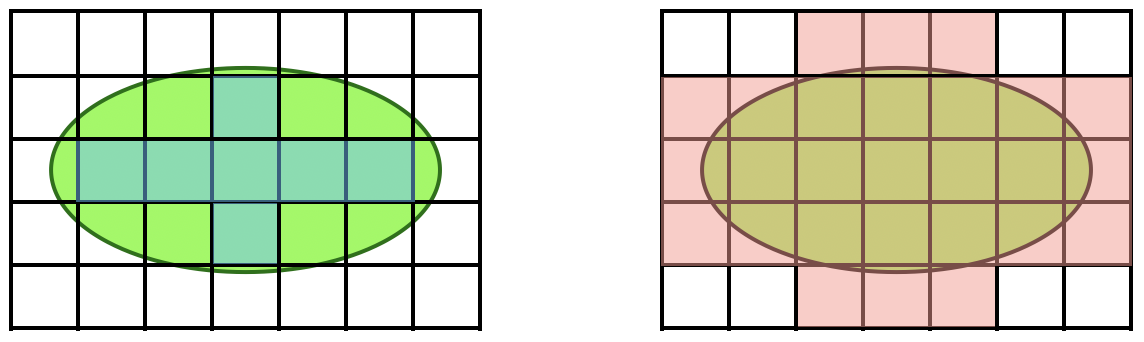
\includegraphics[width=80mm]{calculus12/cover.png}
 \end{center}
\end{figure}

図形に含まれる正方形は$7$個, 図形と共通部分を持つ正方形は$27$個, であるから
$$
7 \le S \le 27. 
$$

\end{frame}

%%%%%%%%%%%%%%%%%%%%%%%%%%%%%%%%%%%%%%%%%%%%%%%%%%%%%%%%%%%%%%%%%%%%%%%%%%%%%%%%%%%%%%%
%%%%%%%%%%%%%%%%%%%%%%%%%%%%%%%%%%%%%%%%%%%%%%%%%%%%%%%%%%%%%%%%%%%%%%%%%%%%%%%%%%%%%%


\begin{frame}
\frametitle{平面図形の正方形分割}
正方形の一辺を半分にして, 面積$1/4$の正方形を用いて近似することを考える. 

\begin{figure}[htbp]
 \begin{center} 
  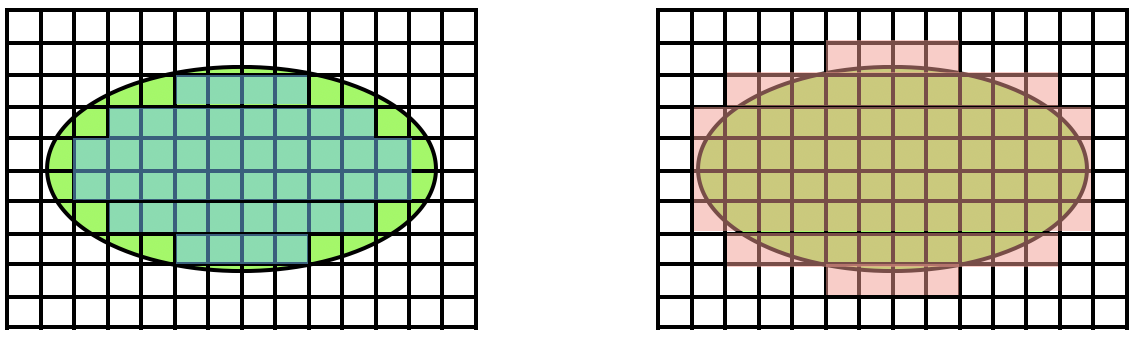
\includegraphics[width=80mm]{calculus12/cover2.png}
 \end{center}
\end{figure}

図形に含まれる正方形は$44$個, 図形と共通部分を持つ正方形は$76$個, であるから
$$
11 \le S \le 19. 
$$

\end{frame}


%%%%%%%%%%%%%%%%%%%%%%%%%%%%%%%%%%%%%%%%%%%%%%%%%%%%%%%%%%%%%%%%%%%%%%%%%%%%%%%%%%%%%%%
%%%%%%%%%%%%%%%%%%%%%%%%%%%%%%%%%%%%%%%%%%%%%%%%%%%%%%%%%%%%%%%%%%%%%%%%%%%%%%%%%%%%%%


\begin{frame}
\frametitle{平面図形の正方形分割}
正方形の一辺をさらに半分にして, 面積$1/16$の正方形を用いて近似することを考える. 

\begin{figure}[htbp]
 \begin{center} 
  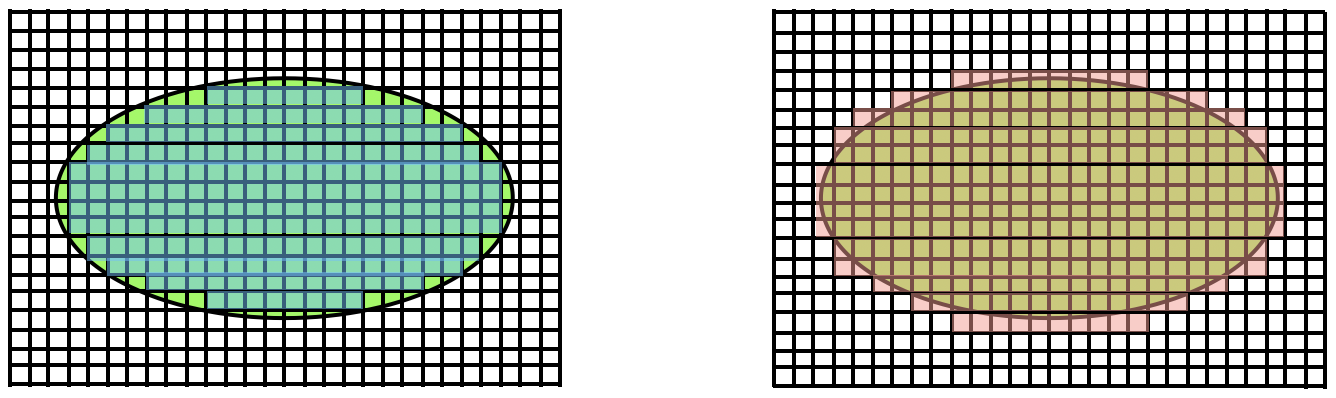
\includegraphics[width=80mm]{calculus12/cover3.png}
 \end{center}
\end{figure}

図形に含まれる正方形は$208$個, 図形と共通部分を持つ正方形は$272$個, であるから
$$
13 \le S \le 17. 
$$

\end{frame}


%%%%%%%%%%%%%%%%%%%%%%%%%%%%%%%%%%%%%%%%%%%%%%%%%%%%%%%%%%%%%%%%%%%%%%%%%%%%%%%%%%%%%%%
%%%%%%%%%%%%%%%%%%%%%%%%%%%%%%%%%%%%%%%%%%%%%%%%%%%%%%%%%%%%%%%%%%%%%%%%%%%%%%%%%%%%%%


%%%%%%%%%%%%%%%%%%%%%%%%%%%%%%%%%%%%%%%%%%%%%%%%%%%%%%%%%%%%%%%%%%%%%%%%%%%%%%%%%%%%%%%
%%%%%%%%%%%%%%%%%%%%%%%%%%%%%%%%%%%%%%%%%%%%%%%%%%%%%%%%%%%%%%%%%%%%%%%%%%%%%%%%%%%%%%


\begin{frame}
\frametitle{平面図形の正方形分割}
面積が$1/2^n$の正方形を用いて近似することを考える. 

\begin{figure}[htbp]
 \begin{center} 
  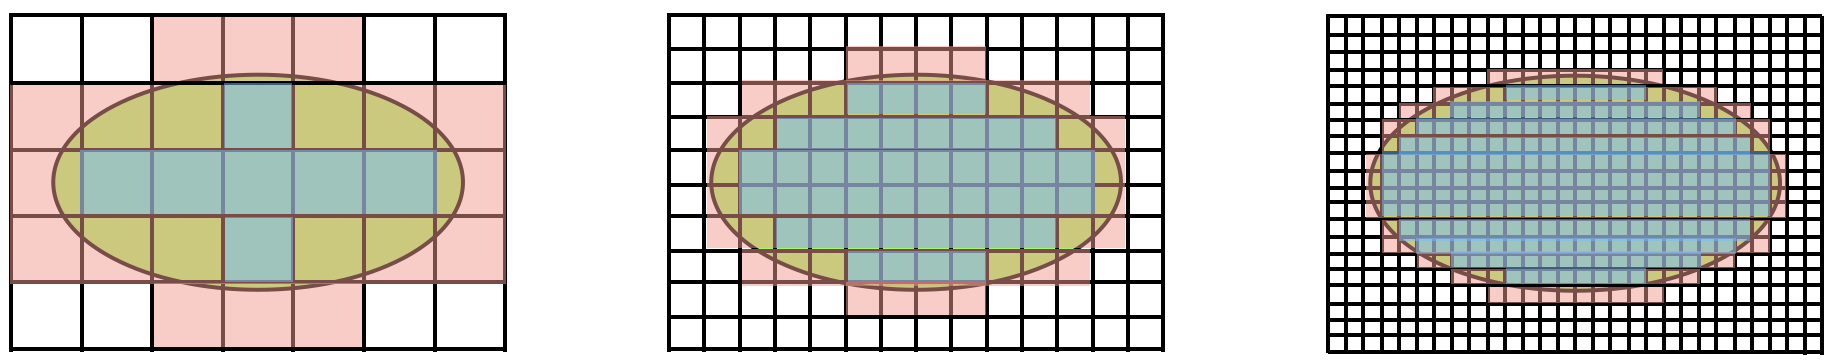
\includegraphics[width=100mm]{calculus12/cover4.png}
 \end{center}
\end{figure}

図形に含まれる正方形の面積の合計$s_n$を内部面積, 図形と共通部分を持つ正方形の面積の合計$S_n$を外部面積という.  
図形の面積が存在すれば
$$
s_1 \le s_2 \le s_3 \le \dots \le S \le \dots \le S_3 \le S_2 \le S_1
$$
正方形を小さくすることで, 内側と外側からの図形の面積の近似精度が上がると考えられる. 


\end{frame}


%%%%%%%%%%%%%%%%%%%%%%%%%%%%%%%%%%%%%%%%%%%%%%%%%%%%%%%%%%%%%%%%%%%%%%%%%%%%%%%%%%%%%%%
%%%%%%%%%%%%%%%%%%%%%%%%%%%%%%%%%%%%%%%%%%%%%%%%%%%%%%%%%%%%%%%%%%%%%%%%%%%%%%%%%%%%%%


\begin{frame}
\frametitle{区分求積法}

\begin{Def}
極限$\displaystyle \lim_{n\to \infty}s_n$と$\displaystyle \lim_{n\to \infty}S_n$が存在し, 
両者が一致するとき図形は\underline{面積確定}, もしくはジョルダン可測と呼ばれ,  
その面積を
$$
S= \lim_{n\to \infty}s_n=\lim_{n\to \infty}S_n
$$
と定義する. 
一般に, 長方形を用いて面積を定義・計算する方法を区分求積法という. 
\end{Def}

面積確定でない図形も存在する. 
実際, 様々な測度(面積の定め方)が存在し, 与えられた図形の面積が定義できるか否かは測度に依存する. 
この講義では上記の意味での面積を考えることにする. 


\end{frame}


%%%%%%%%%%%%%%%%%%%%%%%%%%%%%%%%%%%%%%%%%%%%%%%%%%%%%%%%%%%%%%%%%%%%%%%%%%%%%%%%%%%%%%%
%%%%%%%%%%%%%%%%%%%%%%%%%%%%%%%%%%%%%%%%%%%%%%%%%%%%%%%%%%%%%%%%%%%%%%%%%%%%%%%%%%%%%%

\section{リーマン積分}

\begin{frame}
\frametitle{区分求積法}

区分求積法を用いて, $f(x)=x^2$のグラフ, $x$-軸,直線$x=1$に囲まれた領域の面積$S$を求める. 
区間$[0,1]$を$n$等分して, 各小区間の幅を一辺とする長方形を考える. 
\vspace{-2mm}

\begin{figure}[htbp]
 \begin{center} 
  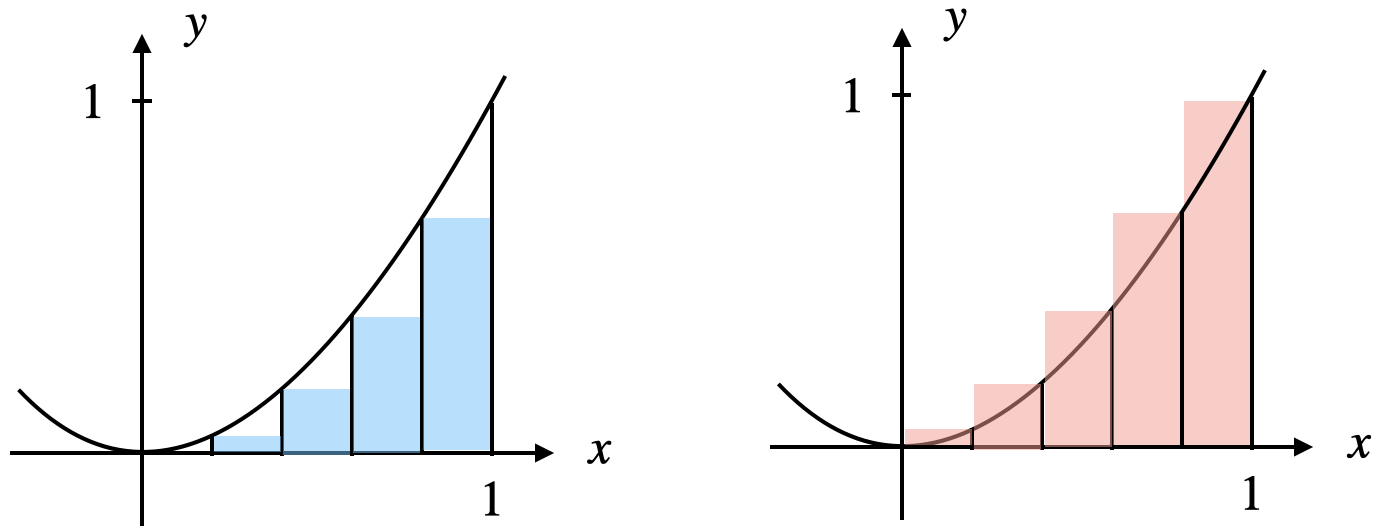
\includegraphics[width=70mm]{calculus12/RiemannSum.png}
 \end{center}
\end{figure}

\vspace{-3mm}

$n=5$のとき
{\small 
\begin{align*}
s_5 &= \frac{1}{5} \cdot \big(\frac{1}{5}\big)^2+\frac{1}{5} \cdot \big(\frac{2}{5}\big)^2+\frac{1}{5} \cdot \big(\frac{3}{5}\big)^2 + \frac{1}{5} \cdot \big(\frac{4}{5}\big)^2
= \frac{1}{5^3}\sum_{k=1}^4 k^2=\frac{6}{25}. \\
S_5 &= \frac{1}{5} \cdot \big(\frac{1}{5}\big)^2+\frac{1}{5} \cdot \big(\frac{2}{5}\big)^2+\frac{1}{5} \cdot \big(\frac{3}{5}\big)^2 
+ \frac{1}{5} \cdot \big(\frac{4}{5}\big)^2 + \frac{1}{5} \cdot \big(\frac{5}{5}\big)^2
= \frac{1}{5^3}\sum_{k=1}^5 k^2=\frac{11}{25}. 
\end{align*}
}

\end{frame}


%%%%%%%%%%%%%%%%%%%%%%%%%%%%%%%%%%%%%%%%%%%%%%%%%%%%%%%%%%%%%%%%%%%%%%%%%%%%%%%%%%%%%%%
%%%%%%%%%%%%%%%%%%%%%%%%%%%%%%%%%%%%%%%%%%%%%%%%%%%%%%%%%%%%%%%%%%%%%%%%%%%%%%%%%%%%%%


\begin{frame}
\frametitle{区分求積法}


\begin{figure}[htbp]
 \begin{center} 
  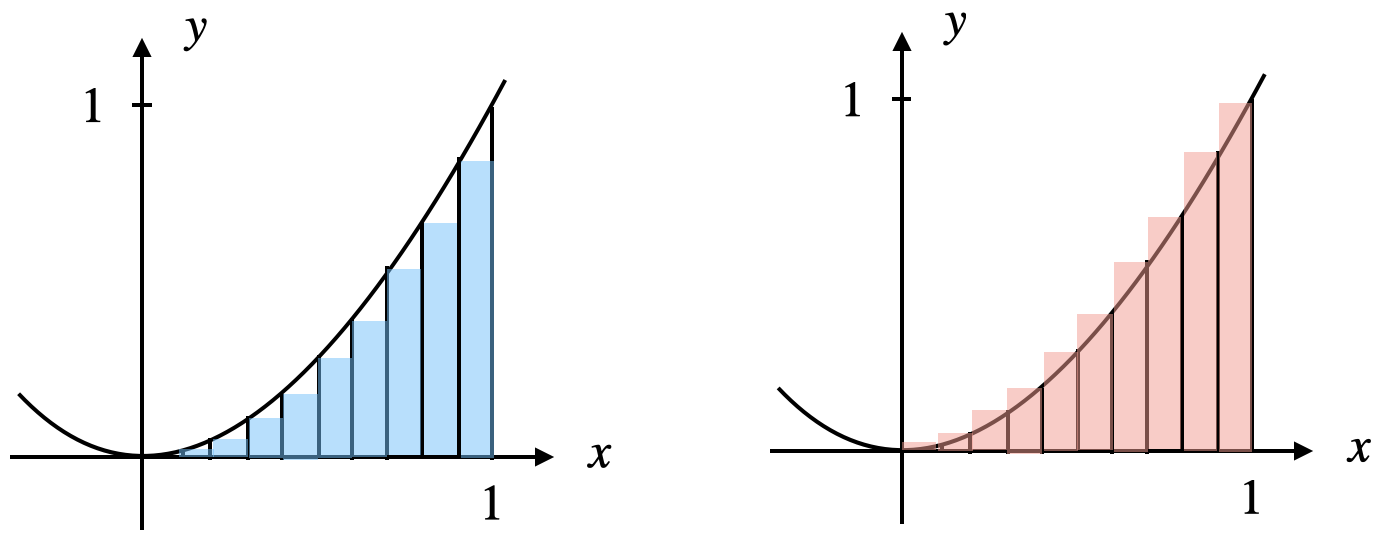
\includegraphics[width=70mm]{calculus12/RiemannSum2.png}
 \end{center}
\end{figure}

\vspace{-3mm}

$n=10$のとき
{\small 
\begin{align*}
s_{10} &= \frac{1}{10} \cdot \big(\frac{1}{10}\big)^2+\frac{1}{10} \cdot \big(\frac{2}{10}\big)^2+\dots 
= \frac{1}{10^3}\sum_{k=1}^9 k^2=\frac{57}{200}. \\
S_{10} &= \frac{1}{10} \cdot \big(\frac{1}{10}\big)^2+\frac{1}{10} \cdot \big(\frac{2}{10}\big)^2+\dots 
= \frac{1}{10^3}\sum_{k=1}^{10} k^2=\frac{77}{200}. 
\end{align*}
}
$S_{10}-s_{10}=1/10$に注意する. 
\end{frame}


%%%%%%%%%%%%%%%%%%%%%%%%%%%%%%%%%%%%%%%%%%%%%%%%%%%%%%%%%%%%%%%%%%%%%%%%%%%%%%%%%%%%%%%
%%%%%%%%%%%%%%%%%%%%%%%%%%%%%%%%%%%%%%%%%%%%%%%%%%%%%%%%%%%%%%%%%%%%%%%%%%%%%%%%%%%%%%


\begin{frame}
\frametitle{区分求積法}

一般に
\begin{align*}
S_n &= \sum_{k=1}^n  \frac{1}{n} \big(\frac{k}{n}\big)^2 = \frac{1}{n^3}  \sum_{k=1}^n k^2 \\
& =  \frac{1}{n^3} \cdot  \frac{1}{6}n(n+1)(2n+1) = \frac{1}{6} (1+\frac{1}{n})(2+\frac{1}{n})
\end{align*}
より$\displaystyle \lim_{n\to \infty}S_n=\frac{1}{3}$. \\
\ \\

一方で, $S_n-s_n=\frac{1}{n}$に注意すると, $\displaystyle \lim_{n\to \infty}s_n=\frac{1}{3}$なので, 
領域の面積は
$$
S= \lim_{n\to \infty}s_n=\lim_{n\to \infty}S_n=\frac{1}{3}.
$$ 

\end{frame}


%%%%%%%%%%%%%%%%%%%%%%%%%%%%%%%%%%%%%%%%%%%%%%%%%%%%%%%%%%%%%%%%%%%%%%%%%%%%%%%%%%%%%%%
%%%%%%%%%%%%%%%%%%%%%%%%%%%%%%%%%%%%%%%%%%%%%%%%%%%%%%%%%%%%%%%%%%%%%%%%%%%%%%%%%%%%%%


\begin{frame}
\frametitle{区分求積法 (補足)}

公式$\displaystyle \sum_{k=1}^n k^2=  \frac{1}{6}n(n+1)(2n+1)$を示す. 恒等式
$$
(k+1)^3-k^3=3k^2+3k+1
$$
の両辺を$k=1$から$n$まで和を取ることを考える. 
\begin{align*}
\text{左辺の和} & = (n+1)^3-n^3+n^3-(n-1)^3+\dots3^3-2^3+2^3-1^3\\
& = (n+1)^3-1=n^3+3n^2+3n. \\
\text{右辺の和} &= 3\sum_{k=1}^n k^2+3\sum_{k=1}^n k+\sum_{k=1}^n 1=  3\sum_{k=1}^n k^2+3\frac{n(n+1)}{2}+n. 
\end{align*}
両辺を整理すると
$$
\sum_{k=1}^n k^2 = \frac{1}{3}(n^3+3n^2+3n-3\frac{n(n+1)}{2}-n)
=  \frac{1}{6}n(n+1)(2n+1). 
$$

\end{frame}


%%%%%%%%%%%%%%%%%%%%%%%%%%%%%%%%%%%%%%%%%%%%%%%%%%%%%%%%%%%%%%%%%%%%%%%%%%%%%%%%%%%%%%%
%%%%%%%%%%%%%%%%%%%%%%%%%%%%%%%%%%%%%%%%%%%%%%%%%%%%%%%%%%%%%%%%%%%%%%%%%%%%%%%%%%%%%%


\begin{frame}
\frametitle{区分求積法}

一般の関数$f(x)$について考える. 
まずは$f(x) \ge 0$のとき, $f(x)$のグラフ, $x$-軸, 直線$x=a$, $x=b$で囲まれた領域を考える. 
区間$[a,b]$を$n$等分する小区間の幅を$\Delta x = (b-a)/n$とおく. 

\vspace{-2mm}

\begin{figure}[htbp]
 \begin{center} 
  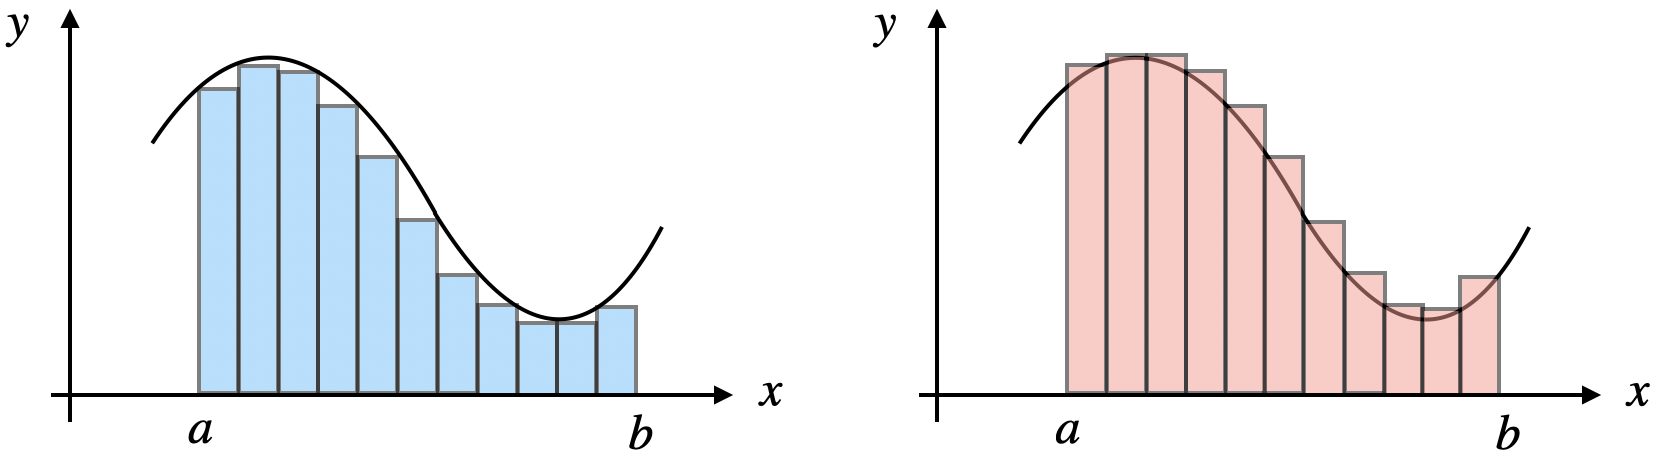
\includegraphics[width=90mm]{calculus12/RiemannSum3.png}
 \end{center}
\end{figure}

\vspace{-2mm}


$k$番目の小区間において, $f(x)$の最小値を与える点を$x_k$, 最大値を与える点を$X_k$とし, 
領域を内側と外側から近似する長方形の集まりの面積をそれぞれ$s_n$, $S_n$とすると
$$
s_n=\sum_{k=1}^nf(x_k)\Delta x, \ \ \ S_n=\sum_{k=1}^nf(X_k)\Delta x
$$




\end{frame}


%%%%%%%%%%%%%%%%%%%%%%%%%%%%%%%%%%%%%%%%%%%%%%%%%%%%%%%%%%%%%%%%%%%%%%%%%%%%%%%%%%%%%%%
%%%%%%%%%%%%%%%%%%%%%%%%%%%%%%%%%%%%%%%%%%%%%%%%%%%%%%%%%%%%%%%%%%%%%%%%%%%%%%%%%%%%%%


\begin{frame}
\frametitle{リーマン和}

\begin{itemize}
\item $s_n=\sum_{k=1}^nf(x_k)\Delta x$は\underline{下ダルブー和}と呼ばれ, $s_1 \le s_2 \le \dots$. 
$$S_*=\lim_{n \to \infty} s_n$$
を区間$[a,b]$における$f(x)$の\underline{下積分}という. 
\item $S_n=\sum_{k=1}^nf(X_k)\Delta x$は\underline{上ダルブー和}と呼ばれ, $S_1 \ge S_2 \ge \dots$. 
$$S^*=\lim_{n \to \infty} S_n$$
を区間$[a,b]$における$f(x)$の\underline{上積分}という. 
\end{itemize}
(有界な単調増加(減少)数列であることから収束が保証される.)

\end{frame}



%%%%%%%%%%%%%%%%%%%%%%%%%%%%%%%%%%%%%%%%%%%%%%%%%%%%%%%%%%%%%%%%%%%%%%%%%%%%%%%%%%%%%%%
%%%%%%%%%%%%%%%%%%%%%%%%%%%%%%%%%%%%%%%%%%%%%%%%%%%%%%%%%%%%%%%%%%%%%%%%%%%%%%%%%%%%%%


\begin{frame}
\frametitle{リーマン積分}


\begin{Def}
下積分$S_*$と上積分$S^*$が一致するとき, $f(x)$は\underline{リーマン積分可能}といい, その値$S_*=S^*$を
$$
\int_a^b f(x)dx
$$
と表す. この値を$f(x)$の\underline{リーマン積分}, もしくは\underline{定積分}という. 
$f(x)$は被積分関数, $[a,b]$は積分区間, $a$は下端, $b$は上端と呼ばれる. 
\end{Def}

一般に, $\sum_{k=1}^nf(x_k^*)\Delta x$の形の和をリーマン和という($x_k^*$は$k$番目の小区間の点). 
$n \to \infty$のとき, リーマン和が$x_k^*$の取り方に依らずある値に収束することとリーマン積分可能性は同値であり, 
その極限値がリーマン積分である.  

\end{frame}


%%%%%%%%%%%%%%%%%%%%%%%%%%%%%%%%%%%%%%%%%%%%%%%%%%%%%%%%%%%%%%%%%%%%%%%%%%%%%%%%%%%%%%%
%%%%%%%%%%%%%%%%%%%%%%%%%%%%%%%%%%%%%%%%%%%%%%%%%%%%%%%%%%%%%%%%%%%%%%%%%%%%%%%%%%%%%%


\begin{frame}
\frametitle{リーマン積分不可能な関数}

不連続関数
$$
f(x)=
\begin{cases}
1 & (x \in \Q)\\
0 & (x \notin \Q)
\end{cases}
$$
を考える. 
任意の小区間において有理数と無理数はどちらも存在するため
\begin{align*}
s_n &= \sum_{k=1}^nf(x_k)\Delta x = \sum_{k=1}^n 0 \cdot \Delta x =0, \\
S_n &= \sum_{k=1}^nf(X_k)\Delta x = \sum_{k=1}^n 1 \cdot \Delta x =n \Delta x = b-a. 
\end{align*}
上積分と下積分が一致しないので, $f(x)$はリーマン積分不可能. \\
\ \\

一方で, 連続な関数はリーマン積分可能であることが知られている. 
\end{frame}



%%%%%%%%%%%%%%%%%%%%%%%%%%%%%%%%%%%%%%%%%%%%%%%%%%%%%%%%%%%%%%%%%%%%%%%%%%%%%%%%%%%%%%%
%%%%%%%%%%%%%%%%%%%%%%%%%%%%%%%%%%%%%%%%%%%%%%%%%%%%%%%%%%%%%%%%%%%%%%%%%%%%%%%%%%%%%%


\begin{frame}
\frametitle{リーマン積分}

\vspace{-3mm}

\begin{figure}[htbp]
 \begin{center} 
  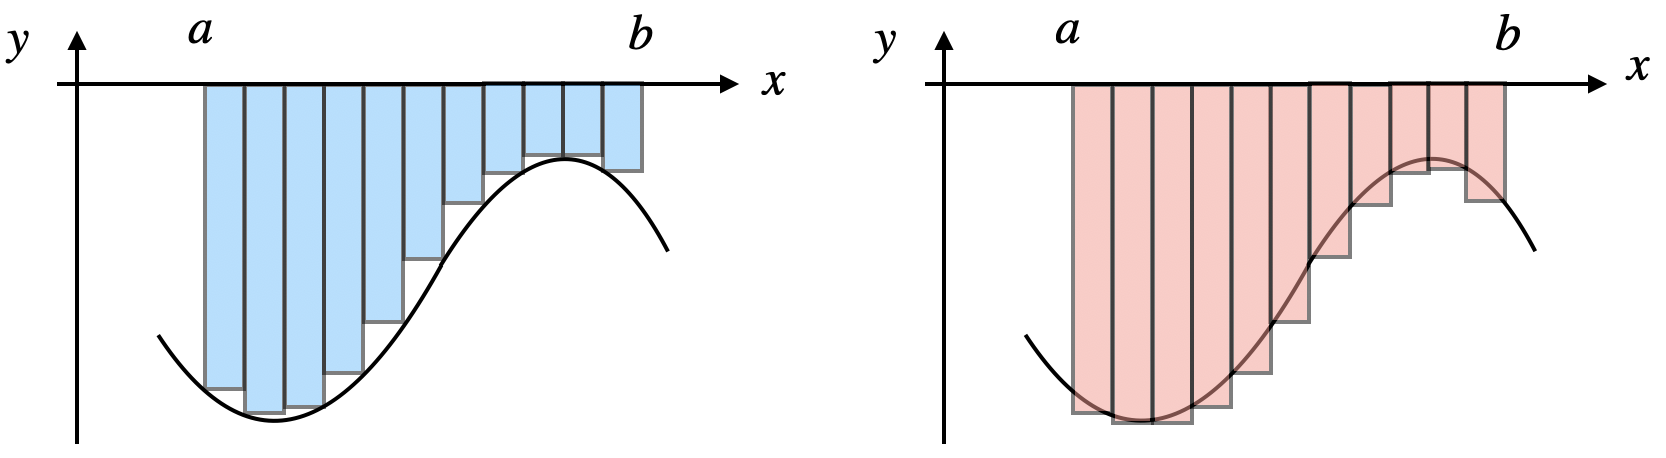
\includegraphics[width=90mm]{calculus12/RiemannSum4.png}
 \end{center}
\end{figure}

\vspace{-3mm}

これまで被積分関数が積分区間上で非負の場合を考えたが, 一般の場合でも定積分は考えられる. 
まず$f(x) \le 0$の場合も同様に積分区間を分割して, 上下のダルブー和を計算する
$$
s_n = \sum_{k=1}^nf(x_k)\Delta x, \ \ \ S_n = \sum_{k=1}^nf(X_k)\Delta x
$$
$x_k$は$k$番目の小区間での$f(x)$の最大値を与える点, $X_k$は最小値を与える点である. 
$\displaystyle \lim_{n\to \infty} s_n = \lim_{n\to \infty} S_n$であるとき, その値を定積分
$\int_a^b f(x)dx$と定める. 


\end{frame}



%%%%%%%%%%%%%%%%%%%%%%%%%%%%%%%%%%%%%%%%%%%%%%%%%%%%%%%%%%%%%%%%%%%%%%%%%%%%%%%%%%%%%%%
%%%%%%%%%%%%%%%%%%%%%%%%%%%%%%%%%%%%%%%%%%%%%%%%%%%%%%%%%%%%%%%%%%%%%%%%%%%%%%%%%%%%%%


\begin{frame}
\frametitle{リーマン積分}


$f(x) \le 0$のとき, $f(x)$の定積分$\int_a^b f(x)dx$は, $f(x)$のグラフ, $x$-軸, 直線$x=a$, $x=b$で囲まれた領域の面積の逆符号を与える. \\
\ \\

一般の関数$f(x)$の定積分は, $f(x)$のグラフ, $x$-軸, 直線$x=a$, $x=b$で囲まれた領域のうち, 
$x$-軸より上の部分の面積を正, 下の部分の面積を負として足し合わせた値として定める. 

\vspace{-1mm}

\begin{figure}[htbp]
 \begin{center} 
  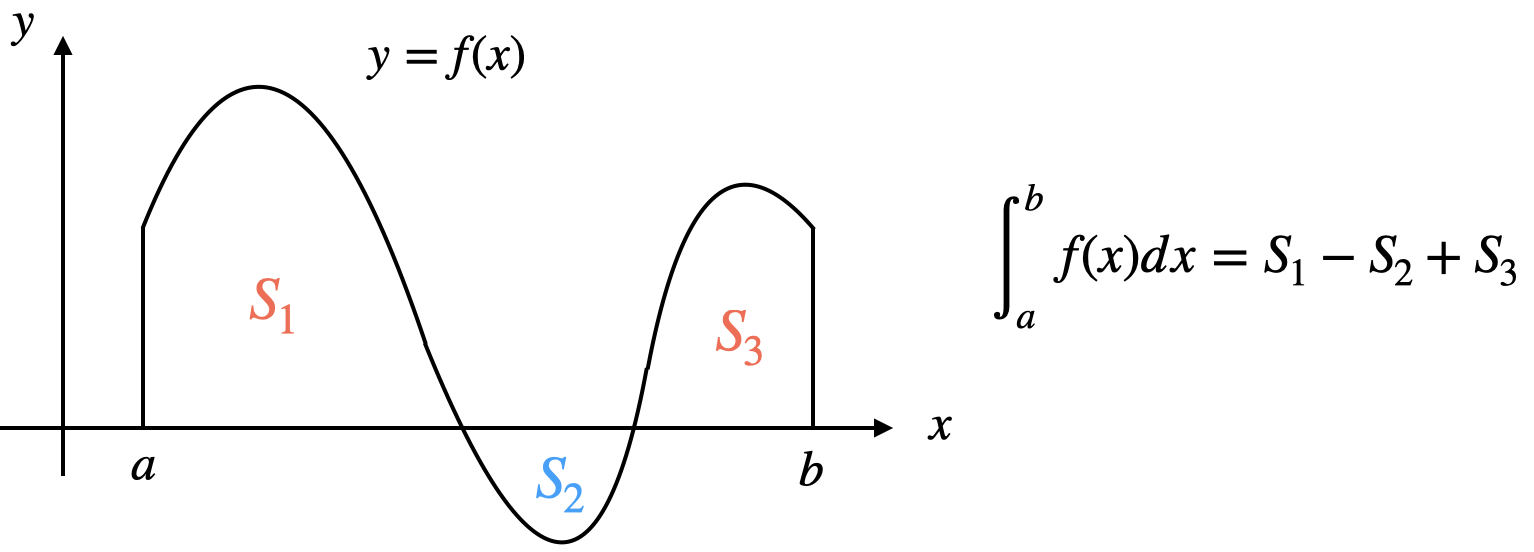
\includegraphics[width=100mm]{calculus12/RiemannInt.png}
 \end{center}
\end{figure}

\vspace{-1mm}

\end{frame}


%%%%%%%%%%%%%%%%%%%%%%%%%%%%%%%%%%%%%%%%%%%%%%%%%%%%%%%%%%%%%%%%%%%%%%%%%%%%%%%%%%%%%%%
%%%%%%%%%%%%%%%%%%%%%%%%%%%%%%%%%%%%%%%%%%%%%%%%%%%%%%%%%%%%%%%%%%%%%%%%%%%%%%%%%%%%%%


\begin{frame}
\frametitle{定積分の性質}

$a,b$の大小が異なる場合も扱えるように, $\int_b^a f(x)dx =- \int_a^b f(x)dx$と定義する. 
定積分は次の性質を持つ. 

\begin{itemize}
\item $\displaystyle \int_a^b (k f(x)+l g(x))dx =  k \int_a^b f(x)dx + l \int_a^b g(x)dx$
\item $\displaystyle f(x) \le g(x) \Longrightarrow  \int_a^b f(x)dx \le \int_a^b g(x)dx$
\item $\displaystyle \big| \int_a^b f(x)dx \big| \le \int_a^b |f(x)|dx \ \ \ (a \le b)$
\item $\displaystyle  \int_a^c f(x)dx = \int_a^b f(x)dx + \int_b^c f(x)dx$
\end{itemize}
ただし$k,l \in \R$. 

\end{frame}


%%%%%%%%%%%%%%%%%%%%%%%%%%%%%%%%%%%%%%%%%%%%%%%%%%%%%%%%%%%%%%%%%%%%%%%%%%%%%%%%%%%%%%%
%%%%%%%%%%%%%%%%%%%%%%%%%%%%%%%%%%%%%%%%%%%%%%%%%%%%%%%%%%%%%%%%%%%%%%%%%%%%%%%%%%%%%%


\begin{frame}
\frametitle{積分の平均値の定理}


\begin{Thm}[積分の平均値の定理]
連続関数$f(x)$に関して
$$
\int_a^b f(x)dx = f(c)(b-a)
$$
を満たす$c \in (a,b)$が存在する. 
\end{Thm}
%証明は連続関数に関する中間値の定理による. 

\begin{figure}[htbp]
 \begin{center} 
  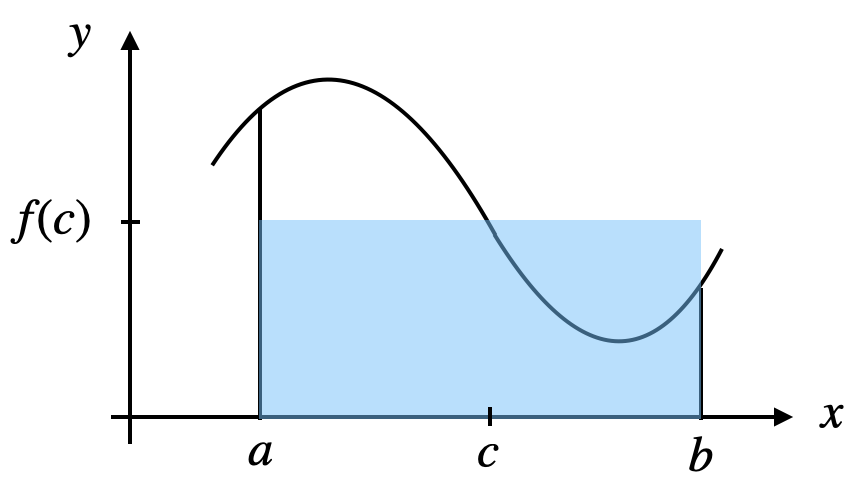
\includegraphics[width=55mm]{calculus12/MeanValueInt.png}
 \end{center}
\end{figure}

\end{frame}


%%%%%%%%%%%%%%%%%%%%%%%%%%%%%%%%%%%%%%%%%%%%%%%%%%%%%%%%%%%%%%%%%%%%%%%%%%%%%%%%%%%%%%%
%%%%%%%%%%%%%%%%%%%%%%%%%%%%%%%%%%%%%%%%%%%%%%%%%%%%%%%%%%%%%%%%%%%%%%%%%%%%%%%%%%%%%%


\begin{frame}
\frametitle{積分の平均値の定理の証明}

ワイエルシュトラスの定理より, 連続関数$f(x)$は$[a,b]$において最大値$M$と最小値$m$を持ち, 
$$
m(b-a) \le \int_a^b f(x)dx \le M(b-a). 
$$
これより
$$
m \le \frac{1}{b-a}\int_a^b f(x)dx \le M.  
$$
連続関数に関する中間値の定理より
$$
\frac{1}{b-a}\int_a^b f(x)dx = f(c)
$$
を満たす$c \in (a,b)$が存在する. 


\end{frame}



%%%%%%%%%%%%%%%%%%%%%%%%%%%%%%%%%%%%%%%%%%%%%%%%%%%%%%%%%%%%%%%%%%%%%%%%%%%%%%%%%%%%%%%
%%%%%%%%%%%%%%%%%%%%%%%%%%%%%%%%%%%%%%%%%%%%%%%%%%%%%%%%%%%%%%%%%%%%%%%%%%%%%%%%%%%%%%%

%%%%%%%%%%%%%%%%%%%%%%%%%%%%%%%%%%%%%%%%%%%%%%%%%%%%%%%%%%%%%%%%%%%%%%%%%%%%%%%%%%%%%%%
%%%%%%%%%%%%%%%%%%%%%%%%%%%%%%%%%%%%%%%%%%%%%%%%%%%%%%%%%%%%%%%%%%%%%%%%%%%%%%%%%%%%%%

\section{定積分と不定積分}

\begin{frame}
\frametitle{微積分学の基本定理}


\begin{Thm}[微積分学の基本定理]
連続関数$f(x)$に対して, 定積分で定まる関数
$$
S(x)=\int_a^x f(t)dt
$$
は$f(x)$の原始関数, つまり
$$
S'(x)= \frac{d}{dx} \int_a^x f(t)dt = f(x).
$$
\end{Thm}
特に
$$
S(c)-S(b)= \int_a^c f(t)dt-\int_a^b f(t)dt = \int_b^c f(t)dt. 
$$

\end{frame}


%%%%%%%%%%%%%%%%%%%%%%%%%%%%%%%%%%%%%%%%%%%%%%%%%%%%%%%%%%%%%%%%%%%%%%%%%%%%%%%%%%%%%%%
%%%%%%%%%%%%%%%%%%%%%%%%%%%%%%%%%%%%%%%%%%%%%%%%%%%%%%%%%%%%%%%%%%%%%%%%%%%%%%%%%%%%%%

\begin{frame}
\frametitle{微積分学の基本定理の証明}


$$
S(x+h)-S(x)=\int_a^{x+h} f(t)dt - \int_a^{x} f(t)dt = \int_x^{x+h} f(t)dt
$$
であるが, 積分の平均値の定理より
$$
\int_x^{x+h} f(t)dt = f(c)h
$$
なる$c \in (x,x+h)$が存在する. 
$h \to 0$とすると, $c \to x$であるので
$$
S'(x)=\lim_{h \to 0} \frac{S(x+h)-S(x)}{h}=\lim_{h \to 0}\frac{f(c)h}{h}=f(x).
$$
(厳密には$h$の正負で場合分けが必要.)

\end{frame}


%%%%%%%%%%%%%%%%%%%%%%%%%%%%%%%%%%%%%%%%%%%%%%%%%%%%%%%%%%%%%%%%%%%%%%%%%%%%%%%%%%%%%%%
%%%%%%%%%%%%%%%%%%%%%%%%%%%%%%%%%%%%%%%%%%%%%%%%%%%%%%%%%%%%%%%%%%%%%%%%%%%%%%%%%%%%%%

\begin{frame}
\frametitle{定積分と不定積分の関係}

\begin{Thm}
$f(x)$の原始関数の一つを$F(x)$とするとき
$$
\int_a^b f(x)dx=F(b)-F(a)=:\big[F(x)\big]_a^b
$$
つまり, 定積分は区分求積法を用いなくとも原始関数から計算可能.  
\end{Thm}
原始関数$F(x)$は無数に存在するが, 先ほど定義した$S(x)$と定数$C$を用いて$F(x)=S(x)+C$と書けるので
$$
F(b)-F(a)=(S(b)+C)-(S(a)+C)=\int_a^bf(x)dx. 
$$

\end{frame}


%%%%%%%%%%%%%%%%%%%%%%%%%%%%%%%%%%%%%%%%%%%%%%%%%%%%%%%%%%%%%%%%%%%%%%%%%%%%%%%%%%%%%%%
%%%%%%%%%%%%%%%%%%%%%%%%%%%%%%%%%%%%%%%%%%%%%%%%%%%%%%%%%%%%%%%%%%%%%%%%%%%%%%%%%%%%%%

\section{定積分の計算}

\begin{frame}
\frametitle{定積分の計算例}

\begin{align*}
\int_1^2(3x^2+4x-1)dx & = \big[x^3+2x^2-x\big]_1^2 \\
& = (2^3+2\cdot 2^2-2)-(1^3+2\cdot 1^2-1) \\
& = 12. 
\end{align*}


\begin{align*}
\int_0^\pi \sin x dx & = \big[ -\cos x\big]_0^\pi \\
& = -\cos \pi - (- \cos 0) \\
& = 2. 
\end{align*}

\end{frame}


%%%%%%%%%%%%%%%%%%%%%%%%%%%%%%%%%%%%%%%%%%%%%%%%%%%%%%%%%%%%%%%%%%%%%%%%%%%%%%%%%%%%%%%
%%%%%%%%%%%%%%%%%%%%%%%%%%%%%%%%%%%%%%%%%%%%%%%%%%%%%%%%%%%%%%%%%%%%%%%%%%%%%%%%%%%%%%


\begin{frame}
\frametitle{定積分の計算例}

\begin{align*}
\int_1^e\frac{1+x^2}{x}dx & = \int_1^e(\frac{1}{x}+x)dx \\
& = \big[ \log x + \frac{1}{2}x^2\big]_1^e \\
& = (\log e + \frac{e^2}{2})-(\log 1 +\frac{1}{2})\\
& = \frac{e^2+1}{2}. 
\end{align*}


\end{frame}


%%%%%%%%%%%%%%%%%%%%%%%%%%%%%%%%%%%%%%%%%%%%%%%%%%%%%%%%%%%%%%%%%%%%%%%%%%%%%%%%%%%%%%%
%%%%%%%%%%%%%%%%%%%%%%%%%%%%%%%%%%%%%%%%%%%%%%%%%%%%%%%%%%%%%%%%%%%%%%%%%%%%%%%%%%%%%%


\begin{frame}
\frametitle{定積分の計算例}


\begin{align*}
\int_0^{2\pi} \sin x dx & = \big[ -\cos x\big]_0^{2\pi} \\
& = -\cos 2\pi - (- \cos 0) \\
& =0. 
\end{align*}

\begin{align*}
\int_0^{2\pi} |\sin x| dx & = \int_0^{\pi} \sin x dx + \int_\pi^{2\pi} (-\sin x) dx \\
& = \big[ -\cos x\big]_0^{\pi} +  \big[ \cos x\big]_\pi^{2\pi} \\
& = -\cos \pi - (- \cos 0) + \cos 2\pi - \cos \pi \\
& =4. 
\end{align*}

\end{frame}



%%%%%%%%%%%%%%%%%%%%%%%%%%%%%%%%%%%%%%%%%%%%%%%%%%%%%%%%%%%%%%%%%%%%%%%%%%%%%%%%%%%%%%%
%%%%%%%%%%%%%%%%%%%%%%%%%%%%%%%%%%%%%%%%%%%%%%%%%%%%%%%%%%%%%%%%%%%%%%%%%%%%%%%%%%%%%%


\section{部分積分}

\begin{frame}
\frametitle{部分積分}

\vspace{-2.7mm}

\begin{Thm}[部分積分の公式] \vspace{-1mm}
$$
\int_a^b f(x)g'(x)dx = \big[f(x)g(x)\big]_a^b - \int_a^b f'(x)g(x)dx
$$
\end{Thm} \vspace{-0.5mm}
実際, 不定積分の部分積分の公式
$$
\int f(x)g'(x)dx = f(x)g(x) - \int f'(x)g(x)dx
$$
より$H(x)=f(x)g(x) - \int_c^x f'(t)g(t)dt$は$ f(x)g'(x)$の原始関数なので \vspace{-1mm}
\begin{align*}
\int_a^b f(x)g'(x)dx &= H(b)-H(a) \\
& = f(b)g(b) - \int_c^b f'(t)g(t)dt - (f(a)g(a) - \int_c^a f'(t)g(t)dt) \\
& = \big[f(x)g(x)\big]_a^b - \int_a^b f'(x)g(x)dx. 
\end{align*}


\end{frame}

%%%%%%%%%%%%%%%%%%%%%%%%%%%%%%%%%%%%%%%%%%%%%%%%%%%%%%%%%%%%%%%%%%%%%%%%%%%%%%%%%%%%%%%
%%%%%%%%%%%%%%%%%%%%%%%%%%%%%%%%%%%%%%%%%%%%%%%%%%%%%%%%%%%%%%%%%%%%%%%%%%%%%%%%%%%%%%


\begin{frame}
\frametitle{部分積分の計算例}


\begin{align*}
\int_1^{e} 4 x \log x dx & = \big[ 2x^2 \log x \big]_1^{e}- \int_1^e 2x^2 \cdot \frac{1}{x}dx \\
& = 2e^2 \log e - 2 \log 1 - \int_1^e2xdx \\
& = 2e^2-\big[x^2\big]_1^e = e^2+1. 
\end{align*}

\begin{align*}
\int_0^{\frac{\pi}{2}} x \cos x  dx & = \big[ x \sin x \big]_0^{\frac{\pi}{2}} - \int_0^{\frac{\pi}{2}} \sin x dx \\
& = \frac{\pi}{2}-0-\big[-\cos x \big]_0^{\frac{\pi}{2}}= \frac{\pi}{2}-1. 
\end{align*}

\end{frame}


%%%%%%%%%%%%%%%%%%%%%%%%%%%%%%%%%%%%%%%%%%%%%%%%%%%%%%%%%%%%%%%%%%%%%%%%%%%%%%%%%%%%%%%
%%%%%%%%%%%%%%%%%%%%%%%%%%%%%%%%%%%%%%%%%%%%%%%%%%%%%%%%%%%%%%%%%%%%%%%%%%%%%%%%%%%%%%

\section{置換積分}

\begin{frame}
\frametitle{置換積分}

\begin{Thm}[置換積分の公式] 
関数$f(x)$の変数$x$が別の変数$t$の$C^1$級関数$x=\phi(t)$として表されるとき
$$
\int_a^b f(x)dx =\int_\alpha^\beta f(\phi(t))\phi'(t)dt
$$
ただし, $\phi(\alpha)=a$,  $\phi(\beta)=b$である. 
\end{Thm}
実際, 不定積分の置換公式
$$
\int f(x)dx =\int f(\phi(t))\phi'(t)dt
$$
より, $F(x)=\int f(x)dx$のとき, $F(\phi(t))$は$ f(\phi(t))\phi'(t)$の原始関数なので
\begin{align*}
\int_\alpha^\beta f(\phi(t))\phi'(t)dt &=  F(\phi(\beta))-F(\phi(\alpha))=F(b)-F(a)=\int_a^b f(x)dx. 
\end{align*}

\end{frame}


%%%%%%%%%%%%%%%%%%%%%%%%%%%%%%%%%%%%%%%%%%%%%%%%%%%%%%%%%%%%%%%%%%%%%%%%%%%%%%%%%%%%%%%
%%%%%%%%%%%%%%%%%%%%%%%%%%%%%%%%%%%%%%%%%%%%%%%%%%%%%%%%%%%%%%%%%%%%%%%%%%%%%%%%%%%%%%


\begin{frame}
\frametitle{置換積分の計算例}

$\int_0^1 \sqrt{1-x^2}dx$を計算する. 
$x=\sin t \ (0 \le t \le \frac{\pi}{2})$と考えると, 
\begin{align*}
\int_0^1 \sqrt{1-x^2}dx & = \int_0^\frac{\pi}{2} \sqrt{1-\sin^2 t} \cos t dt \\
& =  \int_0^\frac{\pi}{2} \cos^2 t dt \\
& =   \int_0^\frac{\pi}{2} \frac{1}{2}(1+\cos 2t)dt \\
& = \Big[\frac{1}{2}(t+\frac{1}{2} \sin 2t) \Big]_0^\frac{\pi}{2}=\frac{\pi}{4}. 
\end{align*}
倍角の公式$\cos 2 \theta = \cos^2 \theta-\sin^2 \theta=2 \cos^2 \theta-1$を用いた. 

\end{frame}

%%%%%%%%%%%%%%%%%%%%%%%%%%%%%%%%%%%%%%%%%%%%%%%%%%%%%%%%%%%%%%%%%%%%%%%%%%%%%%%%%%%%%%%
%%%%%%%%%%%%%%%%%%%%%%%%%%%%%%%%%%%%%%%%%%%%%%%%%%%%%%%%%%%%%%%%%%%%%%%%%%%%%%%%%%%%%%

\section{計算問題}

\begin{frame}
\frametitle{計算問題}

\begin{Prob}
次の定積分を計算せよ. 
\begin{enumerate} 
%\item $\int_1^2(2x^2+3)dx$
\item $\int_0^1x e^{2x}dx$
\item $\int_{0}^\frac{\pi}{3} \tan xdx$
\item $\int_0^1\frac{1}{4-x^2}dx$
\end{enumerate}
\end{Prob}

\end{frame}


%%%%%%%%%%%%%%%%%%%%%%%%%%%%%%%%%%%%%%%%%%%%%%%%%%%%%%%%%%%%%%%%%%%%%%%%%%%%%%%%%%%%%%%
%%%%%%%%%%%%%%%%%%%%%%%%%%%%%%%%%%%%%%%%%%%%%%%%%%%%%%%%%%%%%%%%%%%%%%%%%%%%%%%%%%%%%%


\begin{frame}
\frametitle{計算問題}

%\begin{align*}
%\int_1^2(3x^2-5)dx & = \big[ x^3-5x\big]_1^2=2
%\end{align*}

\begin{align*}
\int_0^1x e^{2x}dx & = \int_0^1 x (\frac{1}{2}e^{2x})'dx = \big[\frac{1}{2}xe^{2x}\big]_0^1- \frac{1}{2} \int_0^1e^{2x}dx \\
& = \frac{1}{2}e^2-\frac{1}{2}\big[\frac{1}{2}e^{2x}\big]_0^1=\frac{1}{4}(e^2+1)
\end{align*}

\begin{align*}
\int_0^\frac{\pi}{3} \tan x dx & =\int_0^\frac{\pi}{3} \frac{\sin x}{\cos x} dx = \int_{1}^\frac{1}{2}\frac{\sin x}{t} \frac{1}{-\sin x}dt \ \ \ (t=\cos x) \\
& = -\big[\log|t|\big]_{1}^\frac{1}{2}= \log 2 
\end{align*}

\begin{align*}
\int_0^1\frac{1}{4-x^2}dx & = \int_0^1\frac{1}{4}(\frac{1}{2-x}+\frac{1}{2+x})dx \\
& = \frac{1}{4}\big[-\log|2-x|+\log|2+x|\big]_0^1=\frac{1}{4}\log 3
\end{align*}
\end{frame}

%%%%%%%%%%%%%%%%%%%%%%%%%%%%%%%%%%%%%%%%%%%%%%%%%%%%%%%%%%%%%%%%%%%%%%%%%%%%%%%%%%%%%%%
%%%%%%%%%%%%%%%%%%%%%%%%%%%%%%%%%%%%%%%%%%%%%%%%%%%%%%%%%%%%%%%%%%%%%%%%%%%%%%%%%%%%%%%












\section{今日のまとめ}
\begin{frame}
\frametitle{まとめ}   


\begin{enumerate}
\item 面積, 区分求積法, リーマン積分, 定積分
\item 微積分学の基本定理, 定積分の計算
\end{enumerate} 


\end{frame}
